\documentclass[12pt,a4paper]{article}

\newif\ifindustry

\industryfalse

%% ---------------------------------
%% |      Additional packages      |
%% ---------------------------------
%% 

\usepackage[utf8]{inputenc}
\usepackage[T1]{fontenc}
\usepackage[a4paper, margin=1in]{geometry} %% margins
\usepackage{natbib} %% References
\usepackage{graphicx} %http://en.wikibooks.org/wiki/LaTeX/Importing_Graphics#Graphics_storage
\usepackage[export]{adjustbox}
\usepackage[absolute,overlay]{textpos}
\usepackage{tikz}
\usepackage{listings}
\usepackage{rotating}
\lstset{
	tabsize=2
}
\usepackage{amsmath,amsfonts,amssymb}	% AMS mathematical facilities, fonts and symbols
\usepackage{lastpage}
\usepackage[bookmarks=true, colorlinks=false]{hyperref} % Links - must be last package

\DeclareGraphicsExtensions{.pdf,.png,.jpg}
\graphicspath{{./figures/}} %Use curly braces for each path to add 

%% ---------------------------------
%% | Information about the report  |
%% ---------------------------------

\newcommand{\mytype}{Laboratoire}
\newcommand{\mytitle}{Laboratoire}
\newcommand{\mystream}{IHDCB335 - Analyse et Modélisation des Systèmes d’Information}

\newcommand{\firststudentname}{Nicolay Matthias}
\newcommand{\secondstudentname}{Demonceau Cédric}

\newcommand{\group}{Groupe 20 HD}

\newcommand{\myyear}{2020}
\newcommand{\duedate}{10/12/2020}

% Describe separation hints here:
\hyphenation{
% Man-age-ment
}


%% ------------------------
%% |    Including files   |
%% ------------------------
% Only files listed here will be included!
% Useful command for partially translating the document (for bug-fixing e.g.)
\includeonly{%
titlepage,
text/game,
text/strat
}

%%%%%%%%%%%%%%%%%%%%%%%%%%%%%%%%%
%% Here, main documents begins %%
%%%%%%%%%%%%%%%%%%%%%%%%%%%%%%%%%
\begin{document}

%% titlepage.tex
%%

% coordinates for the bg shape on the titlepage
\newcommand{\diameter}{20}
\newcommand{\xone}{-15}
\newcommand{\xtwo}{160}
\newcommand{\yone}{15}
\newcommand{\ytwo}{-253}
\newcommand{\myinstitute}{UNamur}

\begin{titlepage}
% bg shape
\begin{tikzpicture}[overlay]
\draw[color=gray]  
 		 (\xone mm, \yone mm)
  -- (\xtwo mm, \yone mm)
 arc (90:0:\diameter pt) 
  -- (\xtwo mm + \diameter pt , \ytwo mm) 
	-- (\xone mm + \diameter pt , \ytwo mm)
 arc (270:180:\diameter pt)
	-- (\xone mm, \yone mm);
\end{tikzpicture}
	\vspace*{3.5cm}
	\begin{center}
		\vspace*{2cm}
		\Large{
			\mytype \\ \mystream
		}\\
		\vspace*{1cm}
		\huge{\firststudentname}\\
		\huge{\secondstudentname}\\
		\vspace*{1cm}
		\huge{\group}\\
		\vspace*{1cm}
		\Large{
			\myinstitute
		}
	\end{center}

\vspace{3cm}
\begin{center}
\large{\date{\today}}
\end{center}

\end{titlepage}

\tableofcontents
\newpage
%% game.tex
%%

%% ==============================
\section{Plateau de Jeu}
\label{sec:game}
%% ==============================

%% question-1.tex
%%

%% ==============================
\subsection{Diagramme de classe minimaliste du jeu}
\label{sec:question-1}
%% ==============================

Voici un diagramme de classe UML qui fixe les éléments principaux du jeu, c'est-à-dire le jeu en lui même, les joueurs, avatars, matchs, rencontres et les mondes.

Le jeu rassemble des joueurs, qui sauvegardent des avatars. Il possède des matchs qui sont constitués de rencontres qui on lieu dans des mondes. Les mondes sont possédés par le jeu.

\begin{figure}[h!]
	\centering
	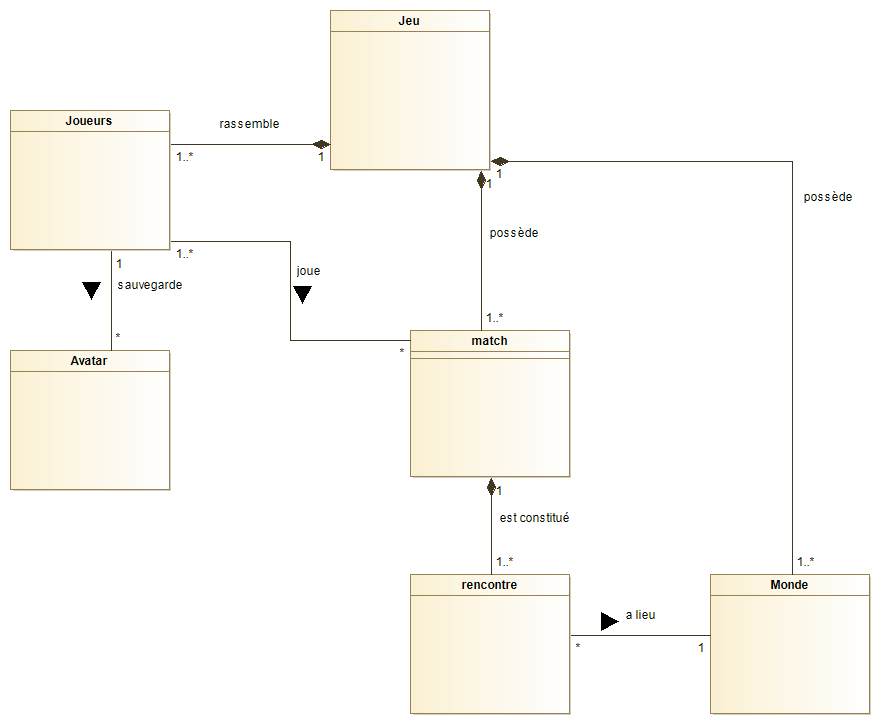
\includegraphics[width=250pt]{assets/diagrammeclassebase}
	\caption{Diagramme de classe des éléments principaux du jeu}
	\label{fig:diagrammeclassebase}
\end{figure}

\newpage
%% question-2.tex
%%

%% ==============================
\subsection{Version enrichie du diagramme de classe du jeu}
\label{sec:question-2}
%% ==============================

Dans cette version du diagramme de classe, la classe Jeu est est maintenant associée a deux nouvelles classes.

La classe \emph{Position}, qui possède deux attributs (x et y), va conserver la position de chaque objet présent pendant le Jeu.

La classe \emph{Personnage}, qui représente les personnages (avatar ou zombie) avec leurs points de vie, ratio d'attaque, leurs effets et leur position. Cette classe à deux sous-classes :
\emph{Zombie} et \emph{Avatar}.

\emph{Avatar} comporte maintenant des aspects normaux et payants, une portée de visibilité, un ratio de défense et un nom. Cette classe est liée à \emph{Détail} qui va garder le détails des matchs et des
opposants rencontrés lors de ceux-ci. Elle est également liée à \emph{Stratégie} qui va contenir la stratégie à appliquer.

La classe \emph{Avatar} est aussi liée à \emph{Rencontre} vu que l'avatar est utilisé lors d'une rencontre. Il possède un \emph{Inventaire}

\emph{Joueurs} est maintenant une classe abstraite contenant un pseudo et s'il à payé pour des aspects supplémentaires. Ses deux sous-classes sont \emph{Physique} qui représente un joueur physique et 
\emph{Machine} qui représente une machine avec un niveau de difficulté.

L'\emph{Avatar} possède également un \emph{Inventaire} qui est composé d'une opération permettant d'ajouter un item à celui-ci. Cet \emph{Inventaire} possède des \emph{Objet}. Ces Objets peuvent être de 4
sous-classes. La première sous-classe \emph{Ramassable} qui peut-être \emph{Nourriture}, \emph{Boisson} et \emph{Munition}. La seconde sous-classe \emph{Orientation}, qui peut être \emph{Carte} ou \emph{Radar}.
La troisième sous-classe \emph{Aide} Qui peut être un \emph{Activable} (une \emph{Cape} ou une \emph{Cotte de maille}), Ou des \emph{Bottes pare-feu}, des \emph{Bottes à crampons} ou un \emph{Kit de plongée}. La quatrième
sous-classe est \emph{Bonus}, qui peut être un \emph{BonusAttaque} ou \emph{BonusDefense}.
Au niveau de la classe \emph{Monde}, elle possède maintenant des \emph{Cases}, qui sont toutes à gauche ou à droite et en haut ou en bas d'un autre. Chaque \emph{Cases} peut être vide ou
alors un \emph{Obstacle}, un \emph{Item} ou le \emph{Graal}. Si elle est un \emph{Obstacle}, celui-ci peut être une \emph{Zone} un \emph{Franchissable} ou un \emph{Infranchissable}.


\begin{sidewaysfigure}
    \centering
	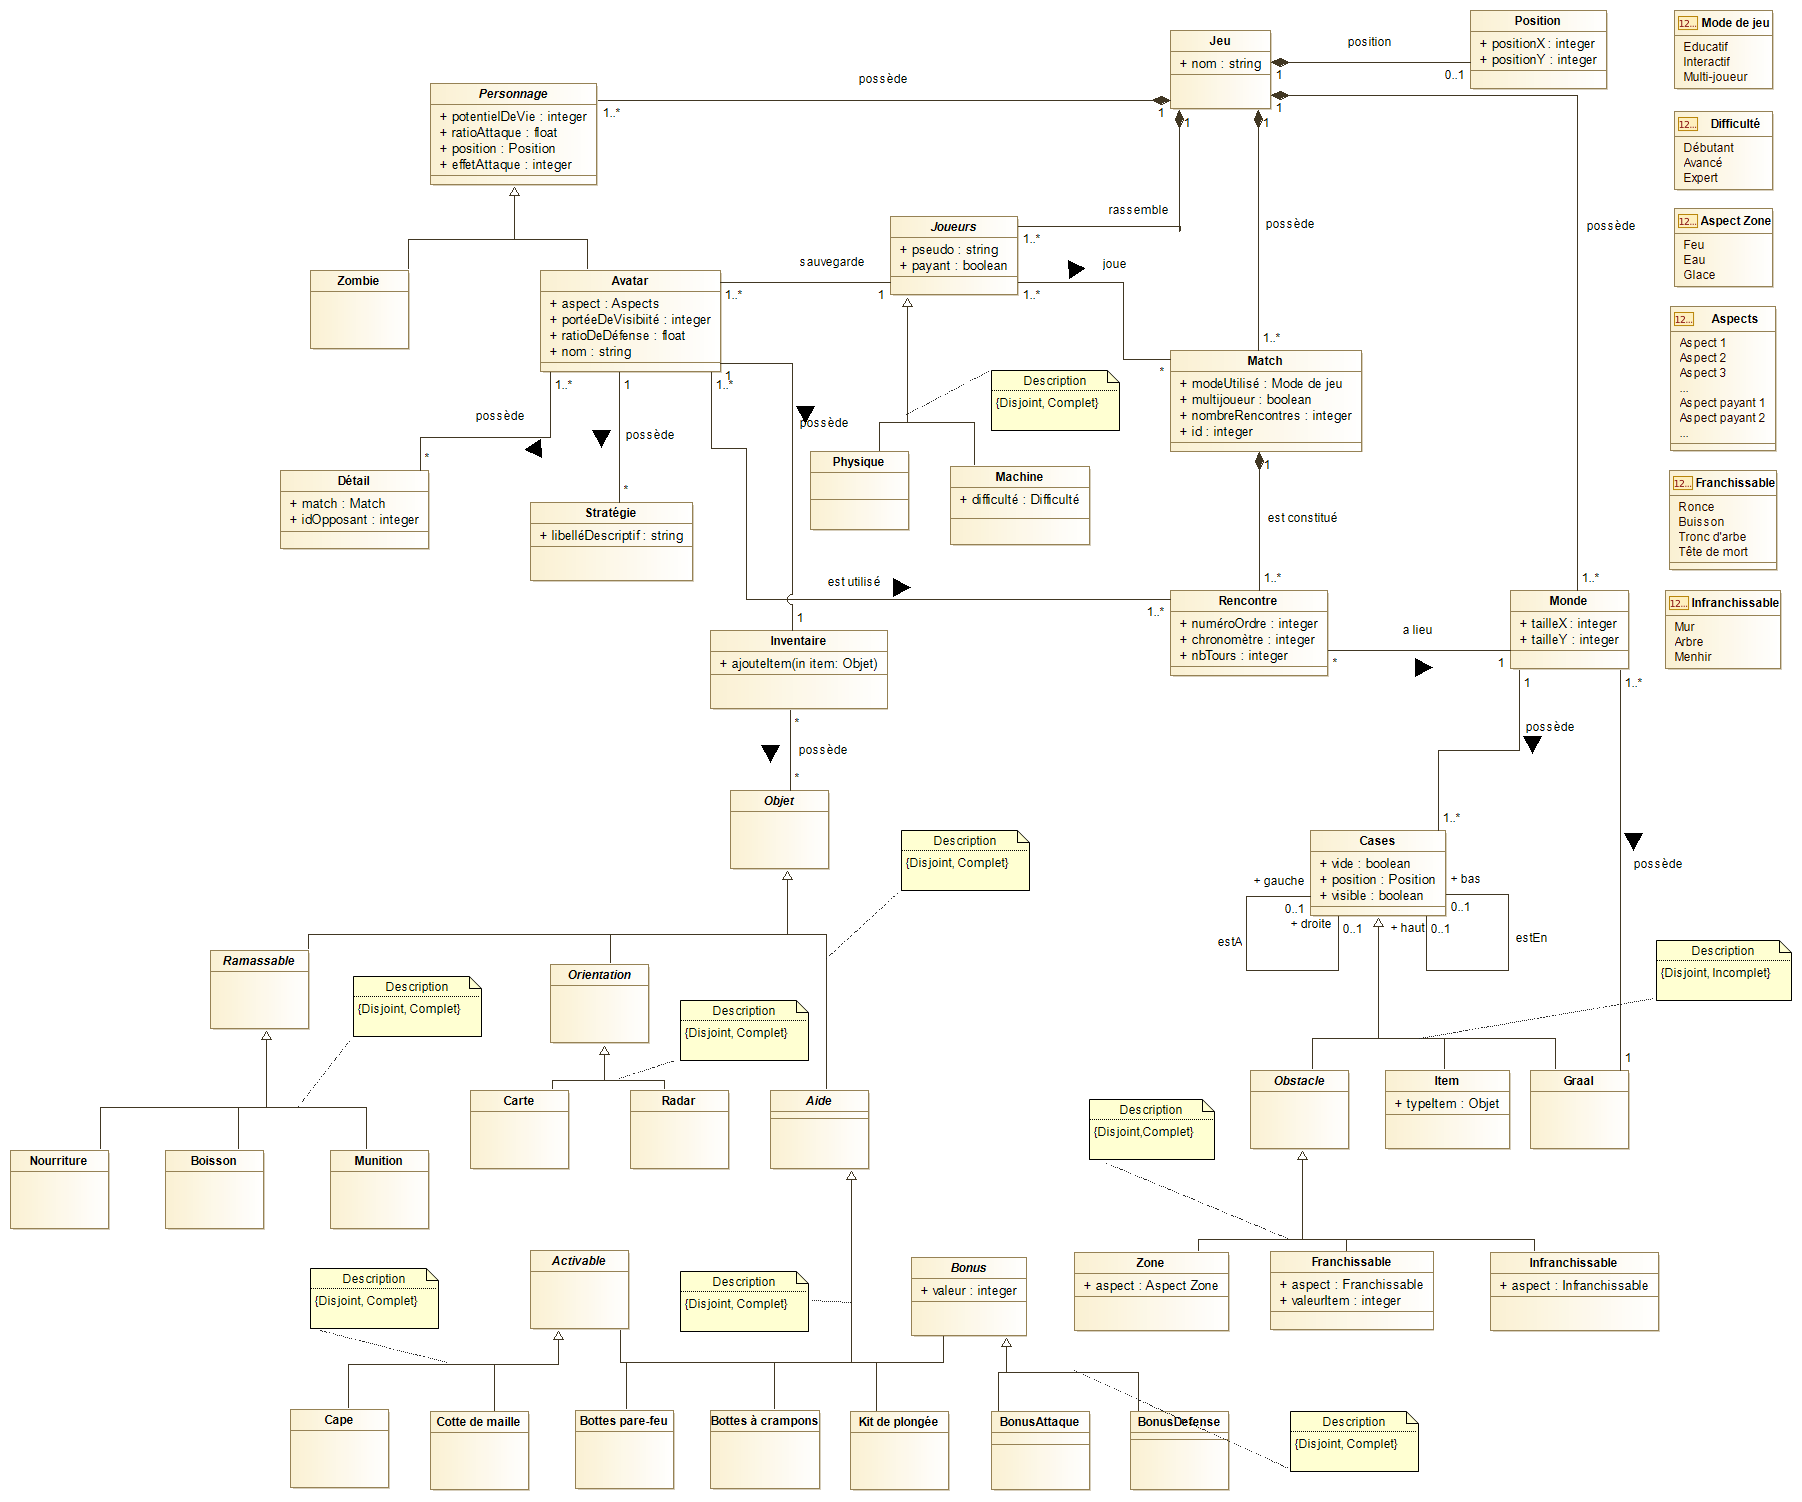
\includegraphics[width=\paperwidth]{assets/Jeu}
	\caption{Diagramme enrichit}
	\label{fig:Jeu}
\end{sidewaysfigure}

\newpage
%% question-3.tex
%%

%% ==============================
\subsection{\textsc{Ocl} - Contraintes d'unicité}
\label{sec:question3}
%% ==============================

Le fait que les matchs sont identifiés de manière unique se caractérise par cette contrainte Ocl:

\begin{lstlisting}[caption=Contrainte sur l'unicité d'un match,captionpos=b,label={lst:match},language=OCL]
context Jeu inv matchUnique :
    self.Match.allInstances -> forall( m1,m2 |
        m1.id <> m2.id implies m1 <> m2)
\end{lstlisting}

La contrainte que des joueurs ont des pseudos différents au sein du jeu se caractérise par cette contrainte :

\begin{lstlisting}[caption=Contrainte sur les pseudos,captionpos=b,label={lst:pseudos},language=OCL]
context Jeu inv pseudoJoueur :
    self.Joueurs.allInstances -> forall( j1,j2 |
        j1.pseudo <> j2.pseudo implies j1 <> j2)
\end{lstlisting}

La contrainte Ocl disant que les personnages/avatars d'un joueur sont nommés différement est exprimée comme suit:

\begin{lstlisting}[caption=Contrainte sur le nom,captionpos=b,label={lst:nomAvatar},language=OCL]
context Joueurs inv nomAvatars :
    self.Avatar.allInstances -> forall( a1,a2 |
        a1.nom <> a2.nom and a1.aspect <> a2.aspect
            implies a1 <> a2)
\end{lstlisting}

La contrainte Ocl obligeant les rencontres à avoir un numéro d'ordre unique est la suivante :

\begin{lstlisting}[caption=Contrainte sur le numéro d'ordre unique,captionpos=b,label={lst:numUnique},language=OCL]
context Match inv ordre :
    self.rencontres.allInstances -> forall( r1,r2 |
        r1.numéroOrdre <> r2.numéroOrdre implies r1 <> r2)
\end{lstlisting}
%% question-4.tex
%%

%% ==============================
\subsection{\textsc{Ocl} - Contraintes OCL du diagramme de classe}
\label{sec:question-4}
%% ==============================


Le fait que le potentiel de vie d'un joueur est toujours positif est caractérisé par la contrainte suivante:

\begin{lstlisting}[caption=Contrainte sur le potentiel de vie,captionpos=b,label={lst:vie},language=OCL]
context Personnage inv vie :
	self.potentielDeVie > 0
\end{lstlisting}

La contrainte exprimant le fait que les ratios d'attaque et de défense sont des ratios s'exprime comme suit:

\begin{lstlisting}[caption=Contrainte sur les ratios,captionpos=b,label={lst:ratios},language=OCL]
context Personnage inv ratios :
	self.ratioAttaque > 0 and self.ratioAttaque < 1
		and
			if self.oclIsTypeOf(Avatar)
				then self.ratioDefense > 0 and self.ratioDefense < 1
			endif
\end{lstlisting}

La contrainte sur la non-parité des rencontres est caractérisée comme suit:

\begin{lstlisting}[caption=Contrainte sur la non-parité des rencontres,captionpos=b,label={lst:impair},language=OCL]
context Match inv nbRencontre :
	self.rencontre.size() % 2 = 1
\end{lstlisting}

La contrainte exprimant que le numéro identifiant la rencontre correspond à son ordre de jeu est la suivante:

\begin{lstlisting}[caption=Contrainte sur l'ordre des rencontres,captionpos=b,label={lst:ordreRencontres},language=OCL]
context Match inv ordone :
	self.rencontre.allInstances -> asOrderedSet()
\end{lstlisting}

La contrainte sur le les 3 types d'items contenu par l'inventaire est représentée dans le diagramme de classe par l'héritage d'\emph{Objet} (figure \ref{fig:Jeu}).

La contrainte qu'un monde ne possède qu'un \emph{Graal} est aussi représentée dans le diagramme de classe par l'association possède entre \emph{Monde} et \emph{Graal} (figure\ref{fig:Jeu}).

La contrainte du fait que les cases ne peuvent excéder la longueur d'un monde est la suivante:

\begin{lstlisting}[caption=Contrainte sur la position des cases,captionpos=b,label={lst:casePos},language=OCL]
context Monde inv posCases :
	self.case.allInstances -> forall ( c |
		c.position.x >= 0 and c.position.x < self.tailleX and
		c.position.y >= 0 and c.position.y < self.tailleY)
\end{lstlisting}

La contrainte  sur la disposition des cases est la suivante :


Le fait que le joueur se trouve dans la case correspondant à sa position absolue est caractérisé par la contrainte suivante :

\begin{lstlisting}[caption=Contrainte sur la position du joueur,captionpos=b,label={lst:posJoueur},language=OCL]
context Avatar inv posAbsolue :
	self.rencontre.monde.case.allInstances -> forall ( c1,c2 |
		self.position.x = c1.position.x and 
		self.position.y = c1.position.y implies
		self.position.x <> c2.position.x and 
		self.position.y <> c2.position.y)
\end{lstlisting}

Le fait que la bordure d'un plateau contienne toujours des éléments infranchissables est caractérisé par la contrainte suivante :

\begin{lstlisting}[caption=Contrainte sur la bordure du plateau,captionpos=b,label={lst:bordurePlat},language=OCL]
context Monde inv Infranchissable :
	self.case.allInstances -> forall(c |
		(c.position.x = 0 and c.position.y <= 0 and 
		c.position.y > self.tailleY or
		c.position.x = self.tailleX - 1 and 
		c.position.y <= 0 and c.position.y > self.tailleY or
		c.position.y = 0 and c.position.x <= 0 and 
		c.position.x > self.tailleX or
		c.position.y = self.tailleY - 1 and c.position.x <= 0 and
		 c.position.x > self.tailleX) implies
			self.case.oclIsTypeOf(Infranchissable)
\end{lstlisting}

La contrainte sur la visibilité est la suivante :

Le fait qu'un personnage ne puisse se trouver sur une case portant un obstacle infranchissable est caractérisé par la contrainte suivante :

\begin{lstlisting}[caption=Contrainte sur la position du joueur sur case infranchissable,captionpos=b,label={lst:caseInfranchissable},language=OCL]
context Monde inv posJoueurCase :
	if self.case.allInstances -> oclIsTypeOf(Infranchissable) and
		self.case.position.x = self.rencontre.avatar.position.x and
		self.case.position.y = self.rencontre.avatar.position.y
	then
		false
	else
		true
	endif
\end{lstlisting}

Le fait que 2 personnages ( zombie compris) ne puissent se trouver sur la même case est caractérisé par la contrainte suivante :

\begin{lstlisting}
context Personnage inv memeCase :
	self.allInstances -> forall ( p1,p2 |
		p1.position.x = p2.position.x and 
		p1.position.y = p2.position.y implies
		p1 = p2)
\end{lstlisting}
%% strat.tex
%%

%% ==============================
\section{Description de Stratégie}
\label{sec:Strat}
%% ==============================

%% question-7.tex
%%

%% ==============================
\subsection{Modélisation du concept de stratégie}
\label{sec:question7}
%% ==============================
Voici un diagramme de classe qui fixe les éléments principaux d'une stratégie :

Une \emph{Stratégie} est composé d'une \emph{vision court terme} et une \emph{vision long terme} qui sont toutes les deux articulées par des objectifs eux même réalisés par des règles.

Une \emph{Stratégie} comporte également des \emph{Déclaration} pouvant être des modules ou des variables.

\begin{figure}[h!]
	\centering
	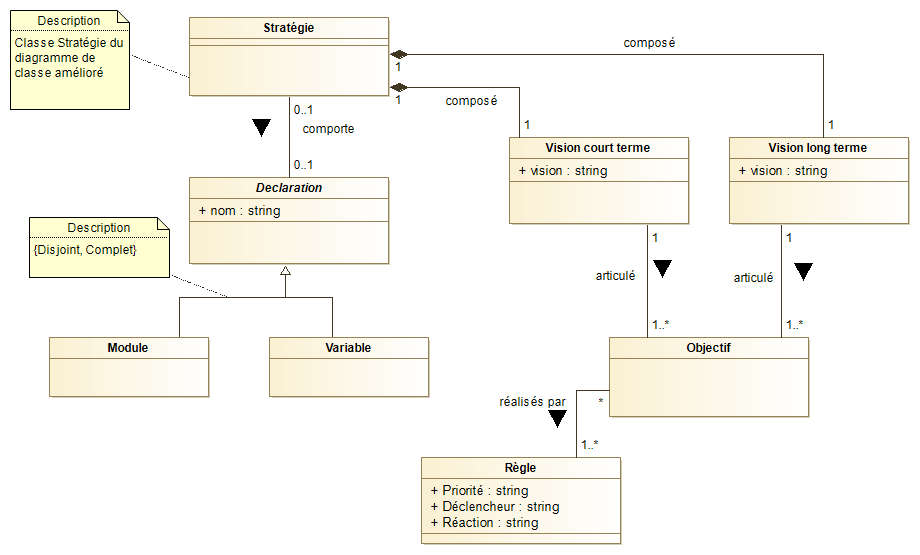
\includegraphics[width=450pt]{assets/strat_base}
	\caption{Diagramme de classe d'une stratégie}
	\label{fig:strategie}
\end{figure}

\newpage
%% question-8.tex
%%

%% ==============================
\subsection{Modélisation du concept de Type}
\label{sec:question8}
%% ==============================

Le concept de \emph{Type} est modélisé de la manière présentée à la figure \ref{fig:type}. La classe \emph{Type} est parent de plusieurs classes présentes dans ce diagramme \emph{Enumération}, \emph{TypePrimitif},\emph{Tableau}. 

On peut remarquer que le type \emph{void} n'est pas considéré comme un type primitif et est donc directement relié à la classe \emph{Type}. 

\begin{figure}
	\centering
	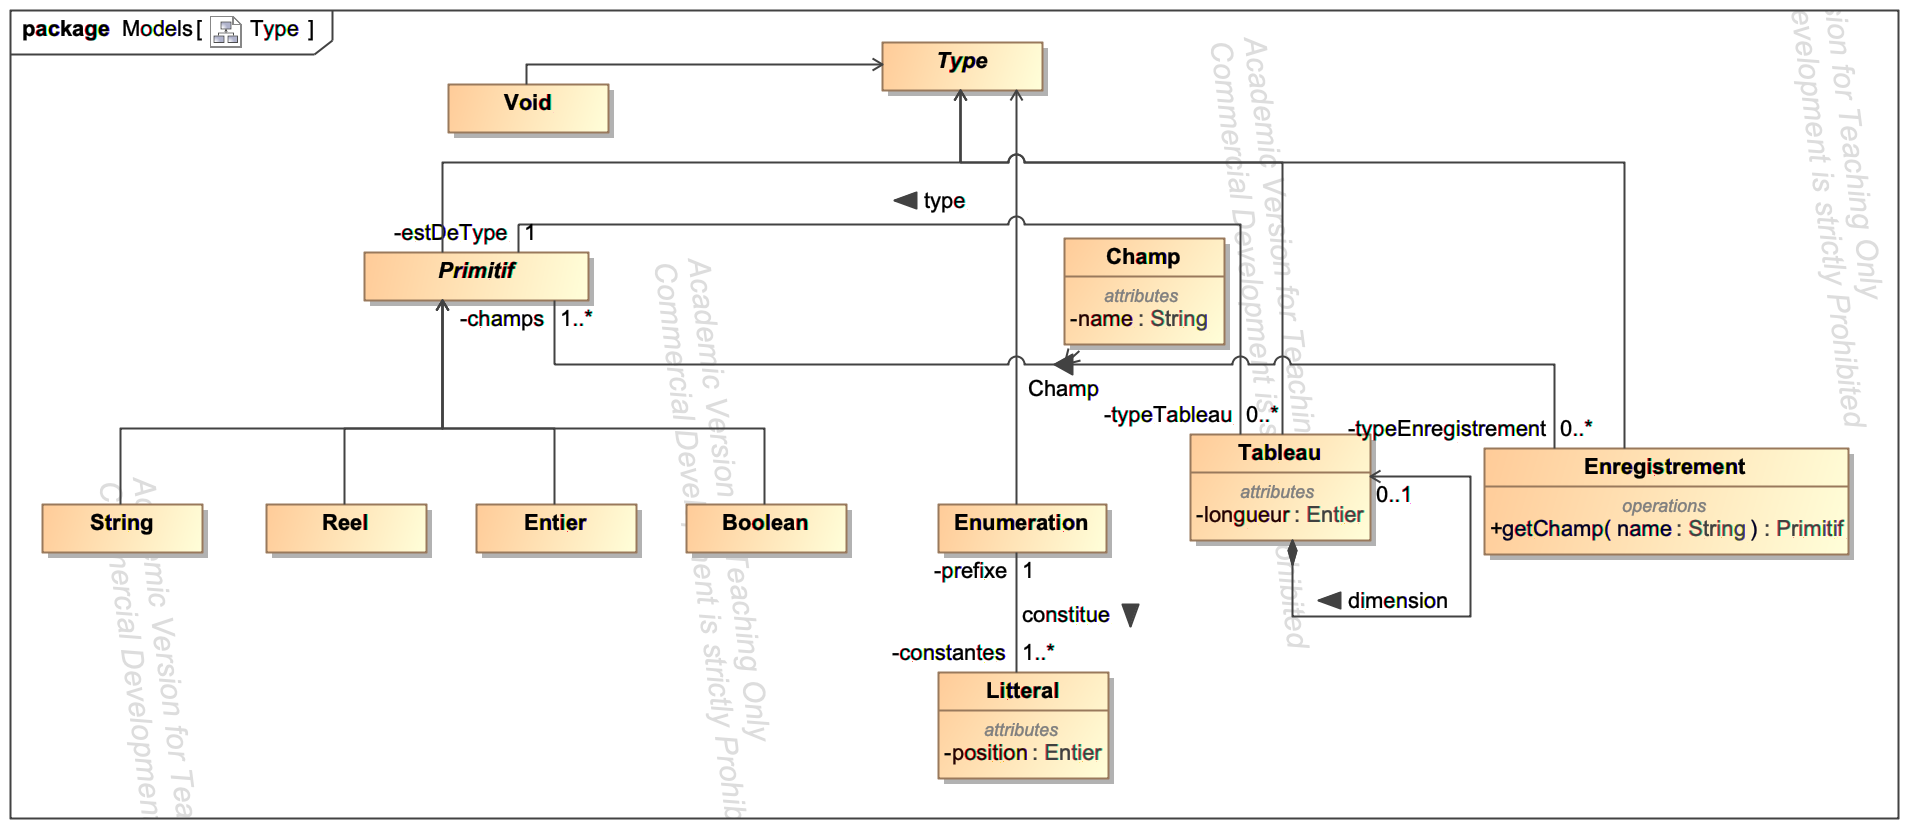
\includegraphics[width=500pt]{assets/class__Type}
	\caption{Diagramme de classe d'un type}
	\label{fig:type}
\end{figure}

%% question-9.tex
%%

%% ==============================
\subsection{Raffinement du concept d'Instruction}
\label{sec:question9}
%% ==============================

Présenté à la figure \ref{fig:instruction}, le raffinement d'\emph{Instruction} montre qu'une \emph{Instruction} possède trois enfants direct (\emph{Composée}, \emph{Affectation} et \emph{AppelProcédure}).

Le diagramme montre aussi qu'une Instruction est enfant de \emph{Déclaration} (comme présenté dans la figure \ref{fig:declaration}). Cela permet d'éviter d'avoir des tableaux de \emph{Void}.

Sur le diagramme, nous pouvons remarquer la classe \emph{Parametres}, celle-ci a été représentée dans la figure \ref{fig:declaration}.  

\begin{figure}
	\centering
	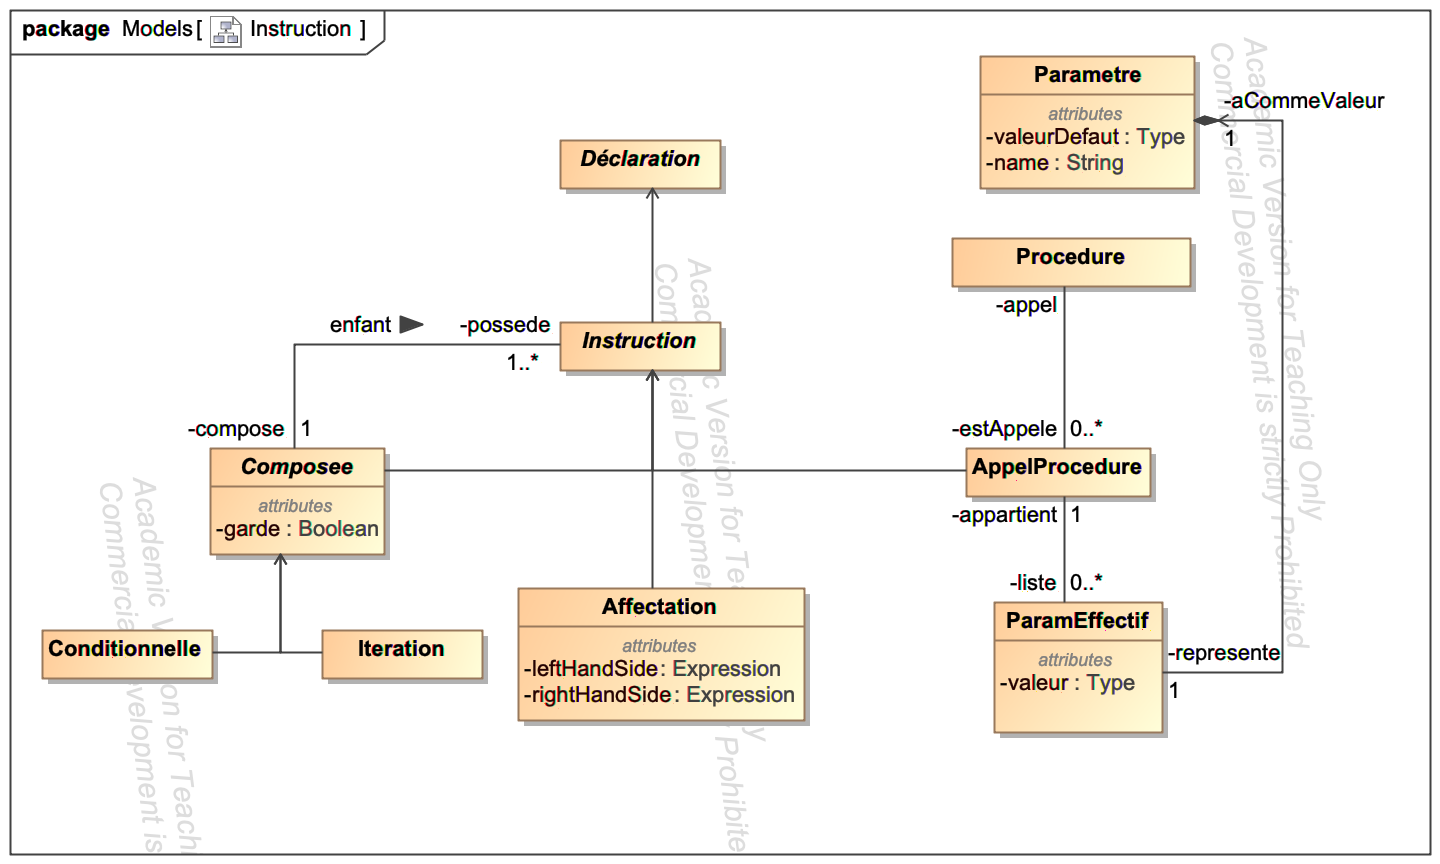
\includegraphics[width=500pt]{assets/class__Instruction}
	\caption{Diagramme de classe d'une instruction}
	\label{fig:instruction}
\end{figure}

%% question-10.tex
%%

%% ==============================
\subsection{Modélisation explicite d'un objectif}
\label{sec:question10}
%% ==============================

Le concept d'objectif est présenté à l'aide de la figure \ref{fig:objectif}. Un \emph{Objectif} est parent de 4 enfants : \emph{Neant} qui est l'objectif par défault. \emph{Combinable} qui est lui même parent de \emph{AllerVers}, \emph{Contourner} et \emph{Eviter}.
\emph{CollecterMax} et \emph{Combattre} sont les deux derniers enfants.
Les \emph{Objectif} sont réalisés par des règles qui possèdent des \emph{Reaction}.

\begin{figure}
	\centering
	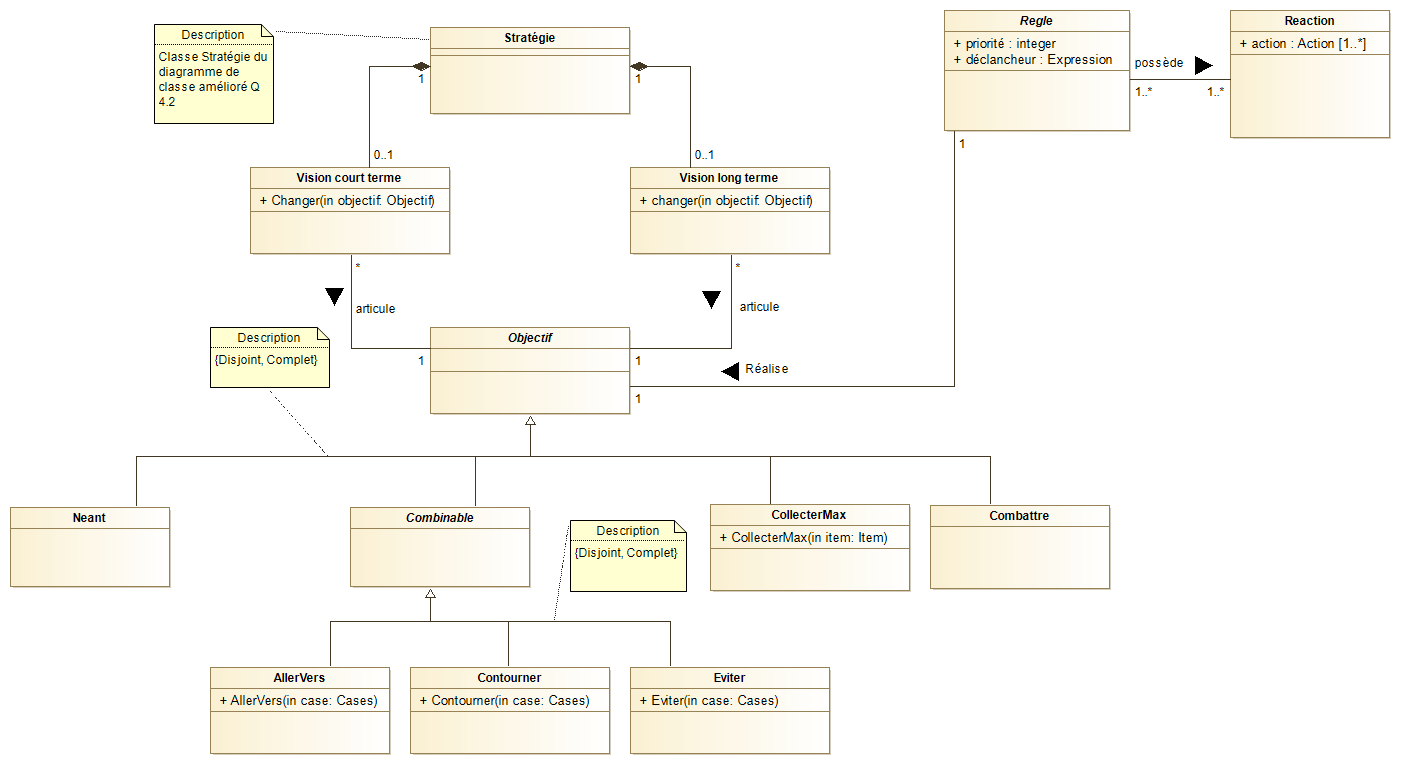
\includegraphics[width=500pt]{assets/class__Objectif}
	\caption{Diagramme de classe d'un objectif}
	\label{fig:objectif}
\end{figure}

%% question-11.tex
%%

%% ==============================
\subsection{Modélisation explicite d'une action}
\label{sec:question11}
%% ==============================

Le concept d'action est présenté à l'aide de la figure \ref{fig:action}. Une \emph{Action} est parent de 6 enfants : \emph{SeDeplacer}, \emph{UtiliserItem}, \emph{Revetir}, \emph{Frapper}, \emph{Tirer} et \emph{ConsulterRadar}.

C'est un personnage qui dispose de ces actions.

\begin{figure}
	\centering
	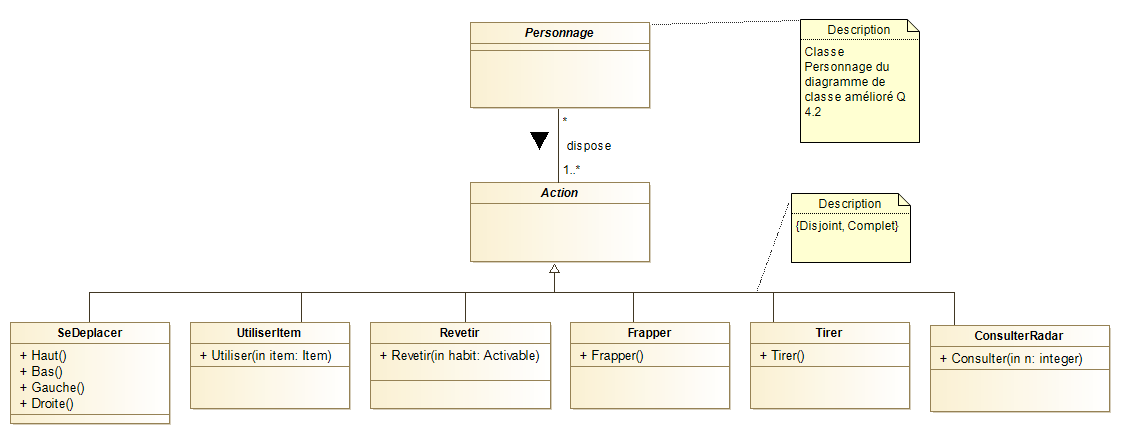
\includegraphics[width=500pt]{assets/class__Action}
	\caption{Diagramme de classe d'une action}
	\label{fig:action}
\end{figure}
%% question-12.tex
%%

%% ==============================
\subsection{Modélisation explicite d'une expression}
\label{sec:question12}
%% ==============================

Le concept d'expression est présenté à l'aide de la figure \ref{fig:expression}. Une \emph{Expression} contient une \emph{Parenthese} et peut prendre la forme de celle-ci. Une Expression peut aussi être un \emph{Literal} qui est une variable, une 
\emph{ExpressionGauche} qui elle même peut être un \emph{AppelVariable} qui invoque une variable, un \emph{AppelChamp} qui provient d'un \emph{Enregistrement}, un \emph{AppelCellule} qui a comme source un \emph{Tableau}. Une \emph{Expression} peut aussi être
un \emph{AppelModule} comportant des \emph{Parametre}, une \emph{Expression Unaire} ou \emph{Binaire} comportant des \emph{Operateur}.

\begin{figure}[h!]
	\centering
	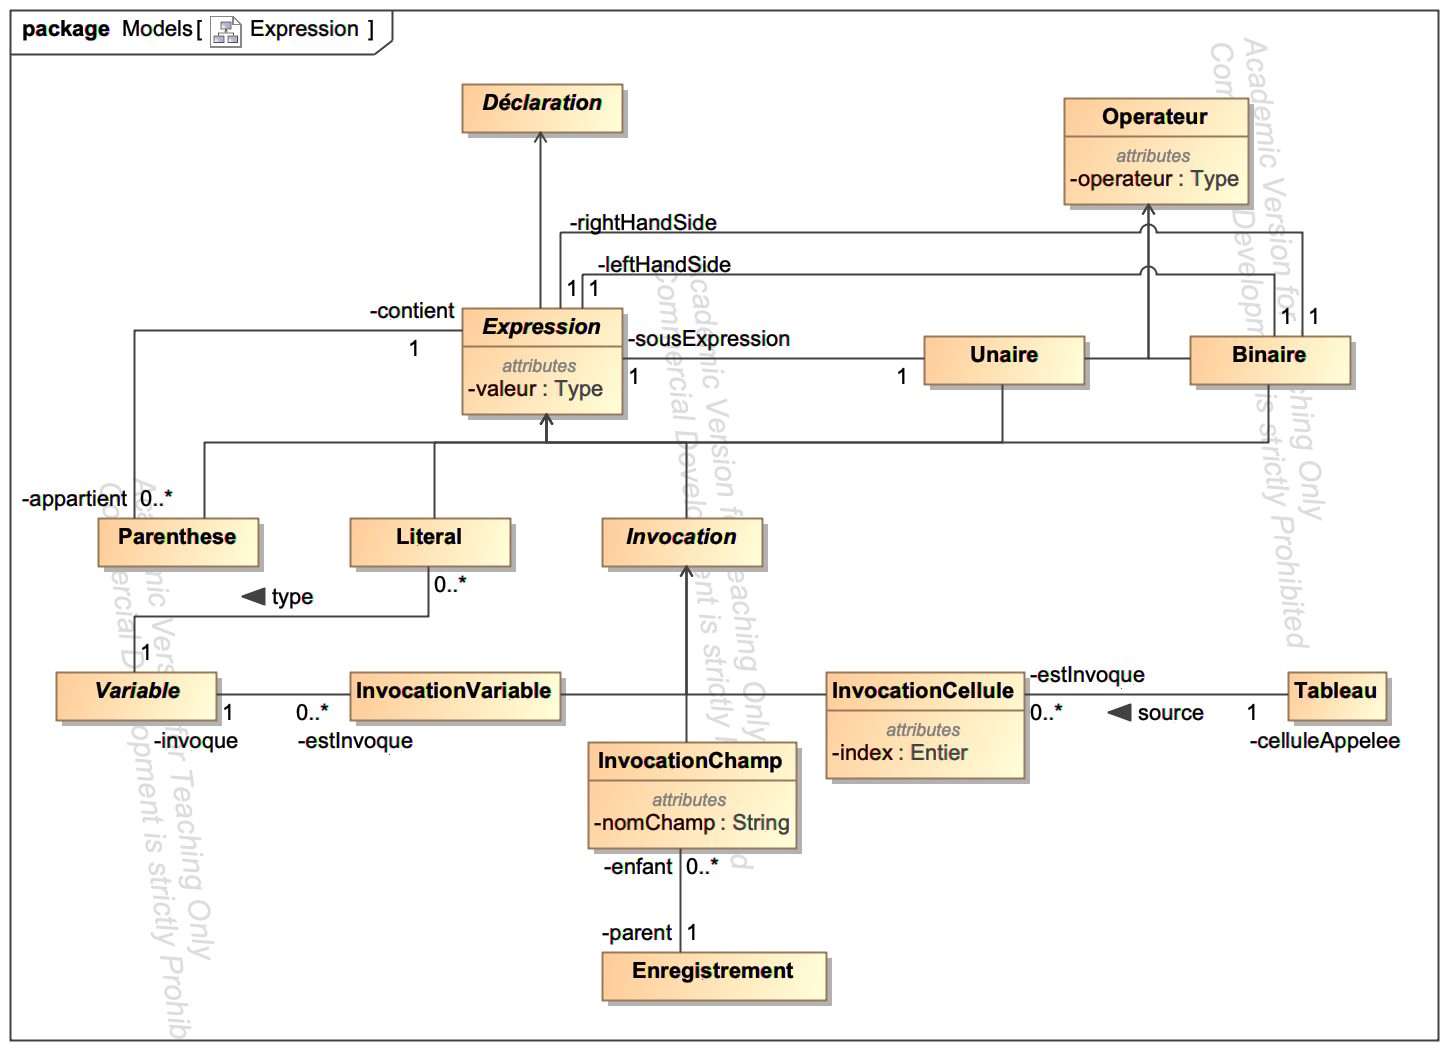
\includegraphics[width=450pt]{assets/class__Expression}
	\caption{Diagramme de classe d'une expression}
	\label{fig:expression}
\end{figure}

\newpage
%% question-13.tex
%%

%% ==============================
\subsection{\textsc{Ocl} - Contrats sur l'opération \emph{type(exp : Expression) : Type}}
\label{sec:question13}
%% ==============================

Dans les différents contrats, la fonction \emph{oclType()} est utilisée. Il s'agit d'une fonction fourni par OCL qui permet d'évaluer le type de l'instance sur laquelle il est appelé \citep{Omg2012}.

Le contrat OCL présenté ci-dessous (Listing \ref{lst:type_type}) spécifie que le type des littéraux est le type qui leur correspond.

\begin{lstlisting}[caption=Le type des littéraux est le type qui leur correspond,captionpos=b,label={lst:type_type},language=OCL]
context Expression::type(exp: Expression)
	post:
		if exp.oclIsTypeOf(Primitif) then
			return exp.oclType()
\end{lstlisting}

Le contrat du listing \ref{lst:type_unaire} indique que le type d'une expression unaire est lié au type de l'opérateur, à condition que sa sous-expression y corresponde.

\begin{lstlisting}[caption=Contrat OCL sur le type unaire,captionpos=b,label={lst:type_unaire},language=OCL]
context Expression::type(exp: Expression)
	post:
		if exp.oclIsTypeOf(Unaire) then
			if exp.operateur.oclIsTypeOf(
				exp.sous-expression.oclType()
			) then
				return exp.operateur.oclType()
\end{lstlisting}

Le contrat OCL suivant (Listing \ref{lst:type_binaire}) défini qu'un type d'une expression binaire est lié au type de son opérateur.

\begin{lstlisting}[caption=Contrat OCL sur le type binaire,captionpos=b,label={lst:type_binaire},language=OCL]
context Expression::type(exp: Expression)
	post:
		if exp.oclIsTypeOf(Binaire) then
			if exp.operateur.oclIsTypeOf(
				exp.leftHandSide.oclType()
			) and exp.operateur.oclIsTypeOf(
				exp.rightHandSide.oclType()
			) then
				return exp.operateur.oclType()
\end{lstlisting}

Le contrat ci-dessous (Listing \ref{lst:type_paranthese}) spécifie que le type d'une expression paranthésée est le type de sa sous-expression.

\begin{lstlisting}[caption=Contrat OCL sur le type parenthèsée,captionpos=b,label={lst:type_paranthese},language=OCL]
context Expression::type(exp: Expression)
	post:
		if exp.oclIsTypeOf(Parenthese) then
			return exp.sous-expression.oclType()
\end{lstlisting}

Le contrat suivant (Listing \ref{lst:type_record}) spécifie que le type d'une expression gauche correspondant à l'accès à un champ est le type de sa déclaration dans l'enregistrement.

\begin{lstlisting}[caption=Contrat OCL sur le type d'un enregistrement,captionpos=b,label={lst:type_record},language=OCL]
context Expression::type(exp: Expression)
	post:
		if exp.oclIsTypeOf(Binaire) then
			if exp.rightHandSide.oclIsTypeOf(InvocationChamp) then
				return exp.rightHandSide.parent
					.getChamp(exp.rightHandSide.nomChamp)
					.oclType()
\end{lstlisting}

Le dernier contrat présenté dans cette section (Listing \ref{lst:type_array}) spécifie que le type d'une expression gauche correspondant à l'accès à une case d'un tableau est le type de la déclaration du tableau.

\begin{lstlisting}[caption=Contrat OCL sur le type d'un tableau,captionpos=b,label={lst:type_array},language=OCL]
context Expression::type(exp: Expression)
	post:
		if exp.oclIsTypeOf(Binaire) then
			if exp.rightHandSide.oclIsTypeOf(InvocationCellule) then
				return exp.rightHandSide.source.type.oclType()
\end{lstlisting}

%% question-14.tex
%%

%% ==============================
\subsection{\textsc{Ocl} - Contraintes d'unicité}
\label{sec:question14}
%% ==============================

La première contrainte d'unicité sur le nom unique des modules est spécifiée comme suit :

\begin{lstlisting}[caption=Nom unique au sein d'une stratégie,captionpos=b,label={lst:nom_unique},language=OCL]
context Strategie inv nomUnique :
	if self.Declaration.allInstances -> oclIsTypeOf(Module) and
		self.Declaration.forall( m1, m2 | m1.nom <> m2.nom)
	then
		true
	else
		false
	endif
\end{lstlisting}

La contrainte sur le nom des variables globales est la suivante :

\begin{lstlisting}[caption=Nom unique d'une variable globale,captionpos=b,label={lst:unique_globale},language=OCL]
context Strategie inv nomVarGlobal :
	if self.Declaration.allInstances ->oclIsTypeOf(Variable) and
		self.Declaration.forall( v1,v2 | v1.nom <> v2.nom)
	then
		true
	else
		false
	endif
\end{lstlisting}

La contrainte sur les variables locales est la suivante :

\begin{lstlisting}[caption=Nom unique des variables locales,captionpos=b,label={lst:nom_locale},language=OCL]
context Module inv uniqueLocale :
	self.Variable.allInstances -> forall(v1,v2 | 
	v1.nom <> v2.nom implies v1 <> v2)
\end{lstlisting}

La contrainte sur les noms des paramètres d'un module est la suivante :

\begin{lstlisting}[caption=Nom unique des paramètres,captionpos=b,label={lst:unique_param},language=OCL]
context Module inv uniqueParam :
	self.Parametre.allInstances -> forall(p1,p2 | 
	p1.nom <> p2.nom implies p1 <> p2)
\end{lstlisting}

La contrainte sur le nom des types soit globalement unique est la suivante :

\begin{lstlisting}[caption=Nom unique des types,captionpos=b,label={lst:type_unique},language=OCL]
context Type inv difNom :
	self.allInstances -> forall( e,t | 
	e.oclIsTypeOf(Enumeration) and t.oclIsTypeOf(Tableau) 
	and e.nom <> t.nom)
\end{lstlisting}
%% question-15.tex
%%

%% ==============================
\subsection{\textsc{Ocl} - Contrats sur l'opération \emph{prec\_mouv() : Déplacement}}
\label{sec:question15}
%% ==============================

Le premier contract OCL (Listing \ref{lst:action_move}) va permet de vérifier que lors d'un déplacement, si on tente d'accéder à une case ou se trouve un obstacle, le déplacement n'est pas effectué.

 \begin{lstlisting}[caption=On empêche le déplacement si la case est occupée par un obstacle,captionpos=b,label={lst:action_move},language=OCL]
context ProcedureAction::right()
	def: player = NiveauEnCours::elements.select(e -> e.name == "Cody"
					and e.oclIsTypeOf(Player))
	post rightObstacle:
		if 	NiveauEnCours::getElementAtPosition(player.Position.X + 1, 
			player.Position.Y).oclIsTypeOf(Obstacle) then
			player.Position.X == player.Position.X@pre and
			player.Position.Y == player.Position.Y@pre
			
context ProcedureAction::left()
	def: player = NiveauEnCours::elements.select(e -> e.name == "Cody"
					and e.oclIsTypeOf(Player))
	post leftObstacle:
		if 	NiveauEnCours::getElementAtPosition(player.Position.X - 1, 
			player.Position.Y).oclIsTypeOf(Obstacle) then
			player.Position.X == player.Position.X@pre and
			player.Position.Y == player.Position.Y@pre
			
context ProcedureAction::up()
	def: player = NiveauEnCours::elements.select(e -> e.name == "Cody"
					and e.oclIsTypeOf(Player))
	post upObstacle:
		if 	NiveauEnCours::getElementAtPosition(player.Position.X , 
			player.Position.Y - 1).oclIsTypeOf(Obstacle) then
			player.Position.X == player.Position.X@pre and
			pPlayer.Position.Y == player.Position.Y@pre
			
context ProcedureAction::down()
	def: player = NiveauEnCours::elements.select(e -> e.name == "Cody"
					and e.oclIsTypeOf(Player))
	post downObstacle:
		if 	NiveauEnCours::getElementAtPosition(player.Position.X, 
			player.Position.Y + 1).oclIsTypeOf(Obstacle) then
			player.Position.X == player.Position.X@pre and
			player.Position.Y == player.Position.Y@pre
\end{lstlisting}

Le contrat OCL (Listing \ref{lst:action_tunnel}) suivant indique que si le joueur accède à une case ou ce trouve un tunnel, il ressort dans la case suivant le dernier mouvement à partir de l'autre tunnel.

\begin{lstlisting}[caption=Contract OCL pour le passage dans un tunnel,captionpos=b,label={lst:action_tunnel},language=OCL]
context ProcedureAction::right()
	def: tunnel : Position
	def: player = NiveauEnCours::elements.select(e -> e.name == "Cody"
					and e.oclIsTypeOf(Player))
	post:
		tunnel = NiveauEnCours::getElementAtPosition(
		player.PositionX + 1, Player.PositionY)
			
		if tunnel.oclIsTypeOf(Tunnel) then
			player.Position.X == tunnel.Sortie.X + 1 
			and player.Position.Y == tunnel.Sortie.Y

context ProcedureAction::left()
	def: tunnel : Position
	def: player = NiveauEnCours::elements.select(e -> e.name == "Cody"
					and e.oclIsTypeOf(Player))
	post:
		tunnel = NiveauEnCours::getElementAtPosition(
		player.PositionX - 1, Player.PositionY)
			
		if tunnel.oclIsTypeOf(Tunnel) then
			player.Position.X == tunnel.Sortie.X - 1
			and player.Position.Y == tunnel.Sortie.Y
			
context ProcedureAction::up()
	def: tunnel : Position
	def: player = NiveauEnCours::elements.select(e -> e.name == "Cody"
					and e.oclIsTypeOf(Player))
	post:
		tunnel = NiveauEnCours::getElementAtPosition(
		player.PositionX, Player.PositionY - 1)
			
		if tunnel.oclIsTypeOf(Tunnel) then
			player.Position.X == tunnel.Sortie.X and
			player.Position.Y == tunnel.Sortie.Y - 1

context ProcedureAction::down()
	def: tunnel : Position
	def: player = NiveauEnCours::elements.select(e -> e.name == "Cody"
					and e.oclIsTypeOf(Player))
	post:
		tunnel = NiveauEnCours::getElementAtPosition(
		player.PositionX, Player.PositionY + 1)
			
		if tunnel.oclIsTypeOf(Tunnel) then
			player.Position.X == tunnel.Sortie.X and
			player.Position.Y == tunnel.Sortie.Y + 1
\end{lstlisting}

Enfin, le dernier contract OCL (Listing \ref{lst:action_jump}) permet d'indiquer que si le joueur saute, il atterit deux cases plus loin dans la même direction. Par contre, s'il y a un obstacle deux cases plus loin, le joueur ne bouge pas.

\begin{lstlisting}[caption=Contract OCL psur le saut,captionpos=b,label={lst:action_jump},language=OCL]
context ProcedureAction::jump()
	def: newPosition : Position
	def: player = Niveau::elements.select(e -> e.name == "Cody" and
					e.oclIsTypeOf(Player))
	post:
		if prec_mouv() == right then
			newPosition = NiveauEnCours::getElementAtPosition(
			player.PositionX + 2, player.PositionY)
			
			if newPosition.oclIsTypeOf(Surface) then
				player.Position.X == player.Position.X@pre + 2 
				and player.Position.Y == player.Position.Y@pre
			else
				player.Position.X == player.Position.X@pre 
				and player.Position.Y == player.Position.Y@pre
		if prec_mouv() == left then
			newPosition = NiveauEnCours::getElementAtPosition(
			player.PositionX - 2, player.PositionY)
			
			if newPosition.oclIsTypeOf(Surface) then
				player.Position.X == player.Position.X@pre - 2 
				and player.Position.Y == player.Position.Y@pre
			else		
				player.Position.X == player.Position.X@pre 
				and player.Position.Y == player.Position.Y@pre
		if prec_mouv() == up then
			newPosition = NiveauEnCours::getElementAtPosition(
			player.PositionX, player.PositionY - 2)
			
			if newPosition.oclIsTypeOf(Surface) then
				player.Position.X == player.Position.X@pre
				and player.Position.Y == player.Position.Y@pre
			else
				player.Position.X == player.Position.X@pre 
				and player.Position.Y == player.Position.Y@pre - 2
		if prec_mouv() == down then
			newPosition = NiveauEnCours::getElementAtPosition(
			player.PositionX, player.PositionY + 2)
			
			if newPosition.oclIsTypeOf(Surface) then
				player.Position.X == player.Position.X@pre 
				and player.Position.Y == player.Position.Y@pre + 2
			else
				player.Position.X == player.Position.X@pre 
				and player.Position.Y == player.Position.Y@pre
\end{lstlisting}
%% question-16.tex
%%

%% ==============================
\subsection{\textsc{Ocl} - Contrats sur l'opération \emph{Expression :: type() : Type}
\label{sec:question16}
%% ==============================

Ce premier contrat porte sur le fait que le type du litéral retourné corresponde au litéral :

\begin{lstlisting}[caption=Contrat \textsc{Ocl} sur le type des litéraux,captionpos=b,label={lst:type_literal},language=OCL]
context Expression :: type() : Type
	post:
		if Type.oclIsTypeOf(TypePrimitif) then
			return Type.oclType()
\end{lstlisting}

Le contrat sur l'opérateur unaire est la suivante :

\begin{lstlisting}[caption=Contrat \textsc{Ocl} sur le type unaire,captionpos=b,label={lst:type_unaire},language=OCL]
context Expression :: type() : Type
	post:
		if Type.oclIsTypeOf(Unaire) then
			if Type.operateur.oclIsTypeOf(
				Type.sous-expression.oclType()
			) then
				return Type.operateur.oclType()
\end{lstlisting}

Le contrat correspondant à l'opérateur binaire est le suivant :

\begin{lstlisting}[caption=Contrat \textsc{Ocl} sur le type binaire,captionpos=b,label={lst:type_binaire},language=OCL]
context Expression :: type() : Type
	post:
		if Type.oclIsTypeOf(Binaire) then
			if Type.operateur.oclIsTypeOf(
				Type.leftHandSide.oclType()
			) and Type.operateur.oclIsTypeOf(
				Type.rightHandSide.oclType()
			) then
				return Type.operateur.oclType()
\end{lstlisting}

Le contrat sur le type de la sous-expression dans une parenthèse est le suivant :

\begin{lstlisting}[caption=Contrat \textsc{Ocl} sur le type paranthésée,captionpos=b,label={lst:type_paranthese},language=OCL]
context Expression :: type() : Type
	post:
		if Type.oclIsTypeOf(Parenthese) then
			return Type.sous-expression.oclType()
\end{lstlisting}

Le contrat sur le type de la déclaration est le suivant :

Le contrat sur le type de renvoi d'une énumération de litéraux est le suivant :

\begin{lstlisting}[caption=Contrat \textsc{Ocl} sur le type de renvoi d'une énum de litéraux,captionpos=b,label={lst:type_énum},language=OCL]
context Expression :: type() : Type
	post :
		if Type.oclIsTypeOf(Litteral)
		then
			return
				Type.est.oslType()
\end{lstlisting}

Le contrat sur le type de retour d'un champ est le suivant :

\begin{lstlisting}[caption=Contrat \textsc{Ocl} sur le type de retour d'un champ,captionpos=b,label={lst:type_champ},language=OCL]
context Expression :: type() : Type
	post :
		if Type.oclIsTypeOf(Champ)
		then
			return
			Type.TypePrimitif.oclType()
\end{lstlisting}

Le contrat sur le type du contenu d'un tableau est le suivant :

\begin{lstlisting}[caption=Contrat \textsc{Ocl} sur le type de retour d'un tableau,captionpos=b,label={lst:type_tableau},language=OCL]
context Expression :: type() : Type
	post :
		if Type.oclIsTypeOf(Tableau)
		then
		 return
		 	Type.est.oclType()
\end{lstlisting}
%% %% question-17.tex
%%

%% ==============================
\subsection{Opération estTraversableGraceAuxItems() : Boolean}
\label{sec:question17}
%% ==============================

La classe de notre diagramme qui pourrait contenir cette opération est Case.

Le contrat de cette définition est le suivant :

\begin{lstlisting}[caption=Contrat \textsc{Ocl} sur l'opération estTraversableGraceAuxItems,captionpos=b,label={lst:operation},language=OCL]
context estTraversableGraceAuxItems(Case,Avatar) : Boolean :
    post :
        if Case.oclIsTypeOf(Zone) and (
            Case.aspect = Feu and
            Avatar.Inventaire.Objet.allInstances() ->
                forall(o | o.oclIsTypeOf(Bottes Pare-Feu))
            or
            Case.aspect = Eau and
            Avatar.Inventaire.Objet.allInstances() ->
                forall(o | o.oclIsTypeOf(Kit De Plongee))
            or
            Case.aspect = Glace and
            Avatar.Inventaire.Objet.allInstances() ->
                forall(o | o.oclIsTypeOf(Bottes a crampon))
        )
        then
            return true
        endif

\end{lstlisting}


%% -----------------
%% |   Main part   |
%% -----------------
\date{}

\pagestyle{plain}

%% --------------------
%% |   Bibliography   |
%% --------------------

% Style
\bibliographystyle{apalike}
\bibliography{refs}

\end{document}
